%% LatexFile made with sciFxt
\documentclass [11pt,spanish]{article}
\usepackage [spanish,activeacute]{babel}
%\usepackage [latin1]{inputenc}
\usepackage[utf8]{inputenc}
\usepackage { amsmath}
\usepackage { upgreek }
\usepackage { mathrsfs }
\usepackage { graphicx }
\usepackage{subfig}
\usepackage { framed,color }
\setlength {\topmargin}{-.5in}
\setlength {\textheight}{9in}
\setlength {\oddsidemargin}{0in}
\setlength {\textwidth}{6.5in}
\begin {document}
\title {Program report}
\author {MACZ\\
Universidad Nacional Aut\'onoma de M\'exico}
\maketitle 

\graphicspath{{./fig/}}

Túnel circular con recubrimiento. Ambos materiales elásticos e isótropos. Tomado del capítulo 3 de Mow y Pao, "The diffraction of elastic waves and dynamic stress concentrations", 1971. 
Ejercicio para incidencia de onda plana P y SV.

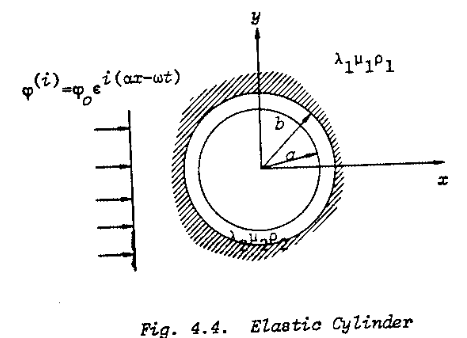
\includegraphics[scale=0.5]{figura}
\begingroup
\fontsize{10pt}{12pt}
\selectfont
\definecolor{shadecolor}{rgb}{0.925,0.925,0.925}
\begin{shaded}
\begin{verbatim}
      module datos
      save
!     real*8, dimension(2), parameter :: rho = (/2.0, 2.0/)
!     real*8, dimension(2), parameter :: nu = (/0.333, 0.333/)
!     real*8, dimension(2), parameter :: bet = (/500.0, 750.0/) !1 medio, 2 liner
      real*8, dimension(2), parameter :: rho = (/2700.0, 7850.0/)
      real*8, dimension(2), parameter :: nu = (/0.25, 0.3/)
      real*8, dimension(2), parameter :: bet = (/3333.333, 3397.23/) !1 medio, 2 liner
      real*8, dimension(2) :: alf
      integer,parameter :: nRes = 120
      real*8, dimension(2) :: radios ! a, b 
      real, parameter :: Qq = 10000.0, Ts = 0.19, Tp = 0.06
      real*8, parameter :: DFREC = 0.66666!0.33
      integer, parameter :: NFREC = 150, nplot = 150, NPTSTIME = 2048
      integer, parameter :: nmax = 500, nfracs = 1
      integer, parameter :: frameInicial = 1, nframes = 168
      real*8, parameter :: Dns = 1.
      complex*16, parameter :: UI = cmplx(0.0d0,1.0d0,8), &
                               UR = cmplx(1.0d0,0.0d0,8), &
                               Z0 = cmplx(0.0d0,0.0d0,8)
      real*8, parameter :: PI = real(4.0d0*ATAN(1.0d0),8)
      logical, parameter :: imprimirEspectros = .true.
      logical, parameter :: hacerSnapshots = .false.
      real :: ventana
      real, parameter :: MeshVecLen = 1.0, giro = 0!-PI/2
      contains
      subroutine set_radios
!     radios(1) = 5.00_8 ! a   : in the liner
!     radios(2) = 5.60_8 ! b   : in the medium
      radios(1) = 5.45_8 ! a   : in the liner
      radios(2) = 5.50_8 ! b   : in the medium
      ventana = 6.5
      end subroutine set_radios
      end module datos
\end{verbatim}
\end{shaded}
\endgroup

\begingroup
\fontsize{10pt}{12pt}
\selectfont
\definecolor{shadecolor}{rgb}{0.925,0.925,0.925}
\begin{shaded}
\begin{verbatim}
      PROGRAM tunelRecub
! Solución analítica de la difración de una onda P incidente 
! en una cavidad cilíndrica circular con recubrimiento
      use datos; use vars_func_of_w; use Hank
      use debug; use RES; use plotter; use fft
      implicit none
      integer :: J,n,et,info,i,ii,ir,minNS
      real*8, pointer :: r,th
      integer, pointer :: reg
      complex*16, dimension(6,6) :: M
      complex*16, dimension(6,2) :: B !P , SV
      integer, dimension(6) :: ipiv 
      complex*16,dimension(nplot) :: pt_RES
      ! terms defined in the appendix (functions)
      complex*16 :: e11,e12,e21,e22,e41,e42,e71,e72,e81,e82,sig0
      real*8,dimension(2) :: BEALF
      character(LEN=4)          :: nom(5)
      character(LEN=9)          :: logflag
      character(LEN=100)        :: titleN,xAx,yAx,CTIT
      
!     complex*16,dimension(:,:),allocatable :: AF
!     complex*16,dimension(:,:),allocatable :: Xbem
!     complex*16,dimension(:),allocatable :: WORKbem
!     real*8,dimension(:),allocatable :: Rbem,Cbem,RWORK
!     real*8 :: RCOND,FERR,BERR
!     character*1 :: EQUED
      
      call set_radios !a,b
      call setup_resu !puntos receptores
      Dt = (1.0) / (real(NPTSTIME) * DFREC)
      eta = radios(2)/radios(1) !b/a
      BEALF(1:2)=SQRT((0.5-NU(1:2))/(1.0-NU(1:2))) !IF POISSON RATIO IS GIVEN
      alf(1:2) = bet(1:2)/BEALF(1:2)
\end{verbatim}
\end{shaded}
\endgroup

\begingroup
\fontsize{10pt}{12pt}
\selectfont
\definecolor{shadecolor}{rgb}{0.925,0.925,0.925}
\begin{shaded}
\begin{verbatim}
      do J=1,NFREC !*********************************************
      FREC=DFREC*real(J); if (J .eq. 1)  FREC = 0.5_8 * DFREC ! Hz
      OME=2.0*PI*FREC !rad/s
!     VEL(1,1:2) = cmplx(alf(1:2)*& 
!                  (1.+1./pi/Qq*log(ome/2./pi)),-1./2./Qq,8)
!     VEL(2,1:2) = cmplx(bet(1:2)*& 
!                  (1.+1./pi/Qq*log(ome/2./pi)),-1./2./Qq,8)
      COME = OME * CMPLX(1., -1./(2.*Qq),8)
      VEL(1,1:2) = cmplx(alf(1:2),(/0.,0./),8)
      VEL(2,1:2) = cmplx(bet(1:2),(/0.,0./),8)
      cp(1:2) => VEL(1,1:2) ! dilatación
      cs(1:2) => VEL(2,1:2) ! corte
      w_c(1:2,1:2) = cOME / VEL(1:2,1:2) !(alfa:beta,reg1:reg2)
      beta(1:2) => w_c(2,1:2) !shear wave number
      alfa(1:2) => w_c(1,1:2) !compressional wave number
      p2(1:2) = (alfa(1:2))**2.0 !compressional wave number (square)
      s2(1:2) = (beta(1:2))**2.0 !shear wave number (square)
      aMU(1:2) = RHO(1:2) * cs(1:2)**2.
      Lambda(1:2) = RHO(1:2)* cp(1:2)**2. - real(2.)* aMU(1:2)
      muR = amu(1)/amu(2) !shear moduli ratio
      gammaP = z0! spacing variable  2.5D
      gammaS = z0! spacing variable
      call makeBessels(minNS,.false.) ! n = -1,0,1,2,...,vm (imprimir)
      do n=0,minNS!nmax*nfracs ! ensamblar matriz 4.26 y terminos independientes
      M(1:6,1:6) = z0; B(1:6,1) = z0; iPIV = 6
\end{verbatim}
\end{shaded}
\endgroup
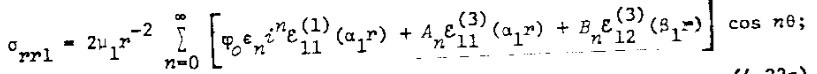
\includegraphics[scale=0.5]{srr1}

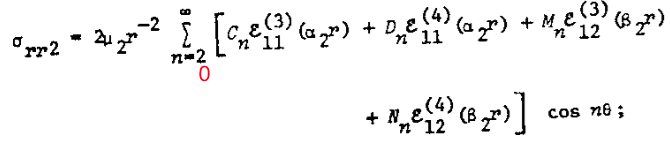
\includegraphics[scale=0.5]{srr2}
\begingroup
\fontsize{10pt}{12pt}
\selectfont
\definecolor{shadecolor}{rgb}{0.925,0.925,0.925}
\begin{shaded}
\begin{verbatim}
      ! sigma_{rr}1 = sigma_{rr}2   @ r = b
      M(1,1) = - muR * e11(3,1,1,2,n)
      M(1,2) = - muR * e12(3,2,1,2,n)
      M(1,3) = e11(3,1,2,2,n)
      M(1,4) = e11(4,1,2,2,n)
      M(1,5) = e12(3,2,2,2,n)
      M(1,6) = e12(4,2,2,2,n) 
      B(1,1) = (1.0) * et(n) * UI**n * muR * e11(1,1,1,2,n)
\end{verbatim}
\end{shaded}
\endgroup
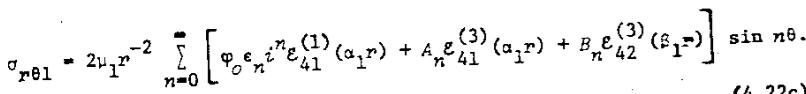
\includegraphics[scale=0.5]{srt1}

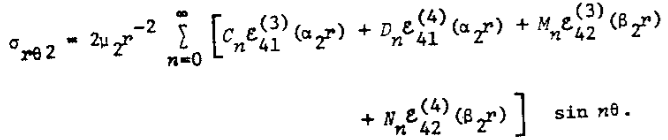
\includegraphics[scale=0.5]{srt2}
\begingroup
\fontsize{10pt}{12pt}
\selectfont
\definecolor{shadecolor}{rgb}{0.925,0.925,0.925}
\begin{shaded}
\begin{verbatim}
      ! sigma_{r th}1 = sigma_{r th}2   @ r = b
      M(2,1) = - muR * e41(3,1,1,2,n)
      M(2,2) = - muR * e42(3,2,1,2,n)
      M(2,3) = e41(3,1,2,2,n)
      M(2,4) = e41(4,1,2,2,n)
      M(2,5) = e42(3,2,2,2,n)
      M(2,6) = e42(4,2,2,2,n)
      B(2,1) = (1.0) * et(n) * UI**n * muR * e41(1,1,1,2,n)

\end{verbatim}
\end{shaded}
\endgroup
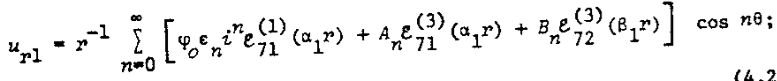
\includegraphics[scale=0.5]{ur1}

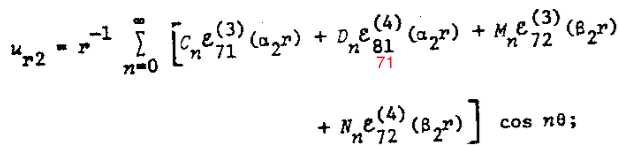
\includegraphics[scale=0.5]{ur2}
\begingroup
\fontsize{10pt}{12pt}
\selectfont
\definecolor{shadecolor}{rgb}{0.925,0.925,0.925}
\begin{shaded}
\begin{verbatim}
      ! u_{r}1 = u_{r}2   @ r = b
      M(3,1) = - e71(3,1,1,2,n) 
      M(3,2) = - e72(3,2,1,2,n) 
      M(3,3) = e71(3,1,2,2,n)
      M(3,4) = e71(4,1,2,2,n) 
      M(3,5) = e72(3,2,2,2,n)
      M(3,6) = e72(4,2,2,2,n)
      B(3,1) = (1.0) * et(n) * UI**n * e71(1,1,1,2,n)
\end{verbatim}
\end{shaded}
\endgroup
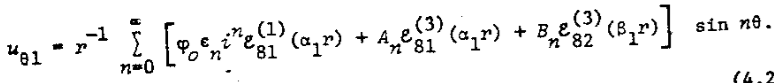
\includegraphics[scale=0.5]{ut1}

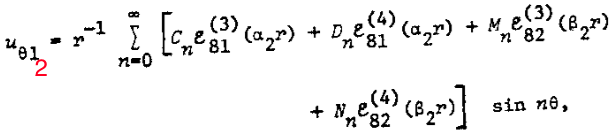
\includegraphics[scale=0.5]{ut2}
\begingroup
\fontsize{10pt}{12pt}
\selectfont
\definecolor{shadecolor}{rgb}{0.925,0.925,0.925}
\begin{shaded}
\begin{verbatim}
      ! u_{th}1 = u_{th}2   @ r = b
      M(4,1) = - e81(3,1,1,2,n) 
      M(4,2) = - e82(3,2,1,2,n) 
      M(4,3) = e81(3,1,2,2,n) 
      M(4,4) = e81(4,1,2,2,n) 
      M(4,5) = e82(3,2,2,2,n)
      M(4,6) = e82(4,2,2,2,n)
      B(4,1) = (1.0) * et(n) * UI**n * e81(1,1,1,2,n)
\end{verbatim}
\end{shaded}
\endgroup
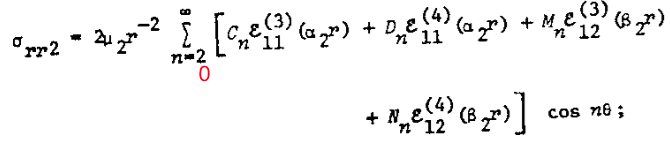
\includegraphics[scale=0.5]{srr2}
\begingroup
\fontsize{10pt}{12pt}
\selectfont
\definecolor{shadecolor}{rgb}{0.925,0.925,0.925}
\begin{shaded}
\begin{verbatim}
      ! sigma_{rr}2 = 0   @ r = a
      M(5,1) = z0
      M(5,2) = z0
      M(5,3) = e11(3,1,2,1,n)
      M(5,4) = e11(4,1,2,1,n)
      M(5,5) = e12(3,2,2,1,n)
      M(5,6) = e12(4,2,2,1,n)
      B(5,1) = z0
\end{verbatim}
\end{shaded}
\endgroup
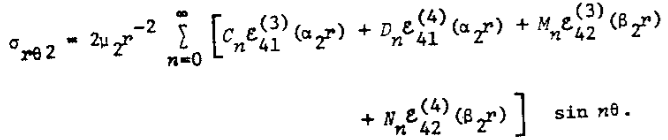
\includegraphics[scale=0.5]{srt2}
\begingroup
\fontsize{10pt}{12pt}
\selectfont
\definecolor{shadecolor}{rgb}{0.925,0.925,0.925}
\begin{shaded}
\begin{verbatim}
      ! sigma_{r th}2 = 0   @ r = a
      M(6,1) = z0
      M(6,2) = z0
      M(6,3) = e41(3,1,2,1,n)
      M(6,4) = e41(4,1,2,1,n)
      M(6,5) = e42(3,2,2,1,n)
      M(6,6) = e42(4,2,2,1,n)
      B(6,1) = z0

\end{verbatim}
\end{shaded}
\endgroup
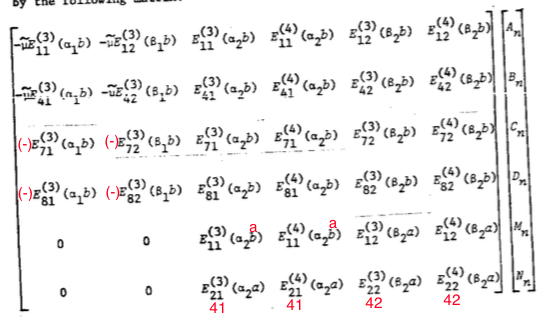
\includegraphics[scale=0.6]{matriz}
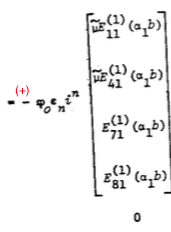
\includegraphics[scale=0.6]{termindep}
\begingroup
\fontsize{10pt}{12pt}
\selectfont
\definecolor{shadecolor}{rgb}{0.925,0.925,0.925}
\begin{shaded}
\begin{verbatim}
!#< r  solve system       . . !#>
      ! driver simple
      call zgesv(6,1,M(1:6,1:6),6,IPIV,B(:,1),6,info)
      
      ! driver experto:
!     call ZGESVX('E','N',6,1,M,6,AF,6,IPIV,EQUED,Rbem, &
!     Cbem,B,6,Xbem,6,RCOND,FERR,BERR,WORKbem,RWORK,INFO)
      
      if(info .ne. 0) then
        write(6,'(A,I0,a,I0)', ADVANCE = "NO") &
        "/",n, " info =",info
        if (info .gt. 6) write(6,'(A)', ADVANCE = "NO") " working precision"
        if (info .le. 6) write(6,'(A)', ADVANCE = "NO") "factor U is exactly singular"
!       stop 1120
        exit
!     else if (abs(B(1,1)) .lt. 0.00000001) then  !NaN
!      write(6,'(A,I0,a)', ADVANCE = "NO") &
!     "trim at",n, " por chiquito abs(B(1)) < 10^{-8}"
!      exit
      else
        write(6,'(A)', ADVANCE = "NO") "."
      end if
!     call showMNmatrixZ(6,1,B,"  A  ",6)     
\end{verbatim}
\end{shaded}
\endgroup

\begingroup
\fontsize{10pt}{12pt}
\selectfont
\definecolor{shadecolor}{rgb}{0.925,0.925,0.925}
\begin{shaded}
\begin{verbatim}
      !#< r elementos mecanicos !#>
      do i = 1,nRes
!      r => Rw(i)%r
       ir = Rw(i)%ir
       th => Rw(i)%th
       reg => Rw(i)%reg
        if (reg .eq. 1) then  !reg 1 in the medium
          Rw(i)%s_rr(J) = Rw(i)%s_rr(J) + &
          (1. * et(n) * UI**n * e11(1,1,1,ir,n) + &
                       B(1,1) * e11(3,1,1,ir,n) + &
                       B(2,1) * e12(3,2,1,ir,n)) * (cos(n * th))
          Rw(i)%s_tt(J) = Rw(i)%s_tt(J) + &
          (1. * et(n) * UI**n * e21(1,1,1,ir,n) + & 
                       B(1,1) * e21(3,1,1,ir,n) + & 
                       B(2,1) * e22(3,2,1,ir,n)) * (cos(n * th))
          Rw(i)%s_rt(J) = Rw(i)%s_rt(J) + &
          (1. * et(n) * UI**n * e41(1,1,1,ir,n) + & 
                       B(1,1) * e41(3,1,1,ir,n) + & 
                       B(2,1) * e42(3,2,1,ir,n)) * (sin(n * th))
          Rw(i)%u_r(J) = Rw(i)%u_r(J) + &
          (1. * et(n) * UI**n * e71(1,1,1,ir,n) + & 
                       B(1,1) * e71(3,1,1,ir,n) + & 
                       B(2,1) * e72(3,2,1,ir,n)) * (cos(n * th))
          Rw(i)%u_t(J) = Rw(i)%u_t(J) + &
          (1. * et(n) * UI**n * e81(1,1,1,ir,n) + & 
                       B(1,1) * e81(3,1,1,ir,n) + & 
                       B(2,1) * e82(3,2,1,ir,n)) * (sin(n * th))
        else if (reg .eq. 2) then !reg 2 in the lining
          Rw(i)%s_rr(J) = Rw(i)%s_rr(J) + &
                      (B(3,1) * e11(3,1,2,ir,n) + &
                       B(4,1) * e11(4,1,2,ir,n) + &
                       B(5,1) * e12(3,2,2,ir,n) + &
                       B(6,1) * e12(4,2,2,ir,n)) * (cos(n * th))
          Rw(i)%s_tt(J) = Rw(i)%s_tt(J) + &
                      (B(3,1) * e21(3,1,2,ir,n) + &
                       B(4,1) * e21(4,1,2,ir,n) + &
                       B(5,1) * e22(3,2,2,ir,n) + &
                       B(6,1) * e22(4,2,2,ir,n)) * (cos(n * th))
          Rw(i)%s_rt(J) = Rw(i)%s_rt(J) + &
                      (B(3,1) * e41(3,1,2,ir,n) + &
                       B(4,1) * e41(4,1,2,ir,n) + &
                       B(5,1) * e42(3,2,2,ir,n) + &
                       B(6,1) * e42(4,2,2,ir,n)) * (sin(n * th))
          Rw(i)%u_r(J) = Rw(i)%u_r(J) + &
                      (B(3,1) * e71(3,1,2,ir,n) + &
                       B(4,1) * e71(4,1,2,ir,n) + &
                       B(5,1) * e72(3,2,2,ir,n) + &
                       B(6,1) * e72(4,2,2,ir,n)) * (cos(n * th))
          Rw(i)%u_t(J) = Rw(i)%u_t(J) + &
                      (B(3,1) * e81(3,1,2,ir,n) + &
                       B(4,1) * e81(4,1,2,ir,n) + &
                       B(5,1) * e82(3,2,2,ir,n) + &
                       B(6,1) * e82(4,2,2,ir,n)) * (sin(n * th))
        end if
      end do! i:nRes
      end do !n
      
      ! términos fuera de la suma:
      do i = 1,nRes
       r => Rw(i)%r
!      th => Rw(i)%th
       reg => Rw(i)%reg
       sig0 = amu(1) * beta(1)**2. !eq 3.15   para hacerlo factor de amplificación
          Rw(i)%s_rr(J) = Rw(i)%s_rr(J) * 2. *amu(reg) / r**2. 
          Rw(i)%s_tt(J) = Rw(i)%s_tt(J) * 2. *amu(reg) / r**2. !/ sig0
          Rw(i)%s_rt(J) = Rw(i)%s_rt(J) * 2. *amu(reg) / r**2. 
          Rw(i)%u_r(J) = Rw(i)%u_r(J) / r 
          Rw(i)%u_t(J) = Rw(i)%u_t(J) / r 
      end do! i:nRes

\end{verbatim}
\end{shaded}
\endgroup

\begingroup
\fontsize{10pt}{12pt}
\selectfont
\definecolor{shadecolor}{rgb}{0.925,0.925,0.925}
\begin{shaded}
\begin{verbatim}
      abscisa(J) = dfrec * 2 * pi * J * radios(1) / cp(1)
      end do !J   
      ! plot curves
      ! end program tunelRecub
      
      
      
      
      
      
      
      
      
      
      
      
      
      
      
      
      
      
      
      
      
      
      
      
      
      
      
      
      
      
      
      
      
      
      
      
      
      
      
\end{verbatim}
\end{shaded}
\endgroup
Se comparan los resultados normalizados para $\eta=1.1$, $r=b$,

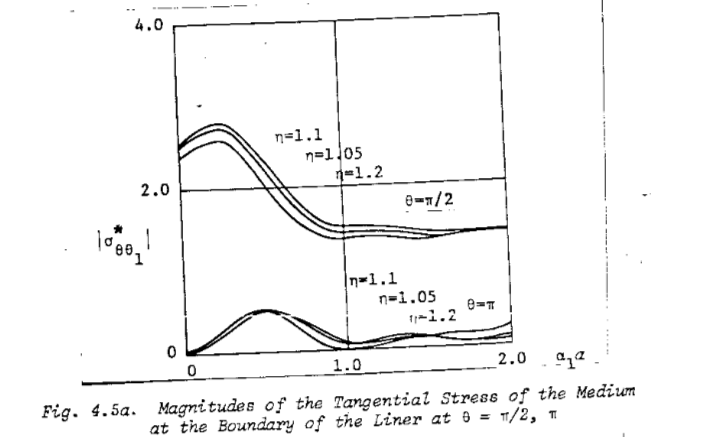
\includegraphics[scale=0.4]{res1}

en $\theta=\pi/2$ y en $\theta=\pi$ respectivamente,

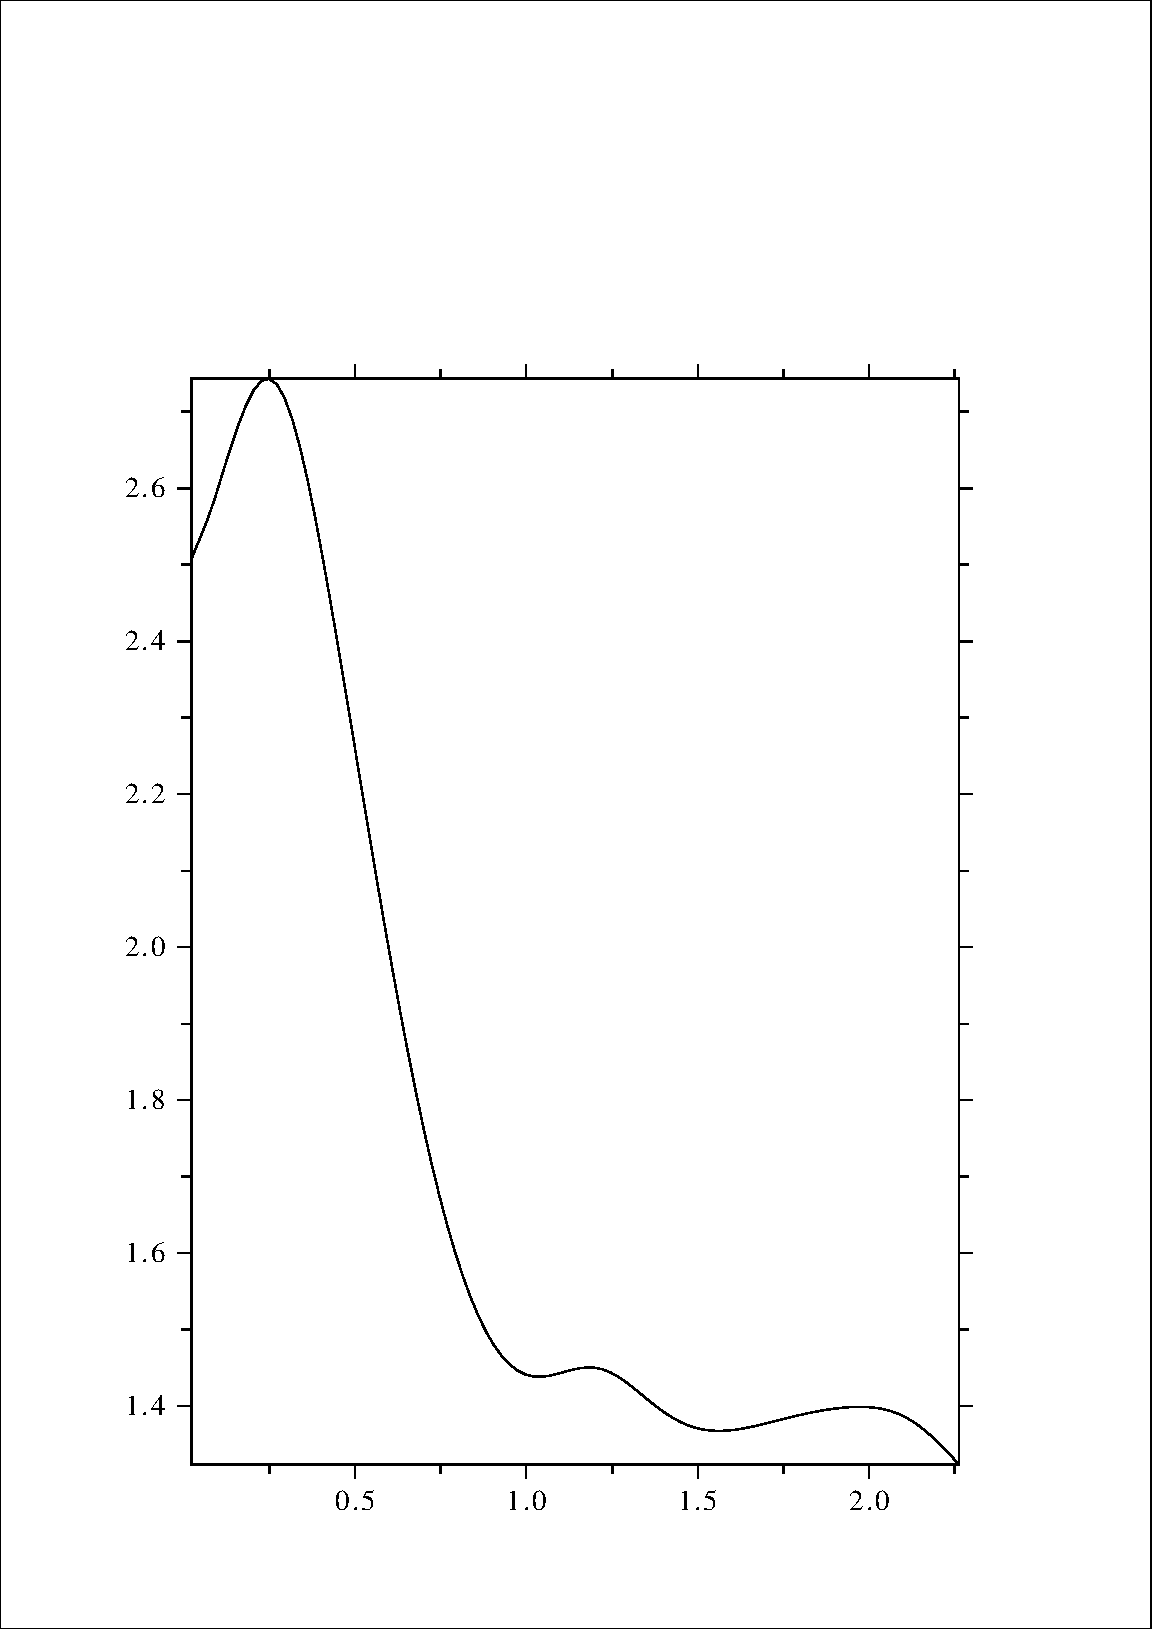
\includegraphics[scale=0.4]{RES_1s_tt1abspi2.pdf}
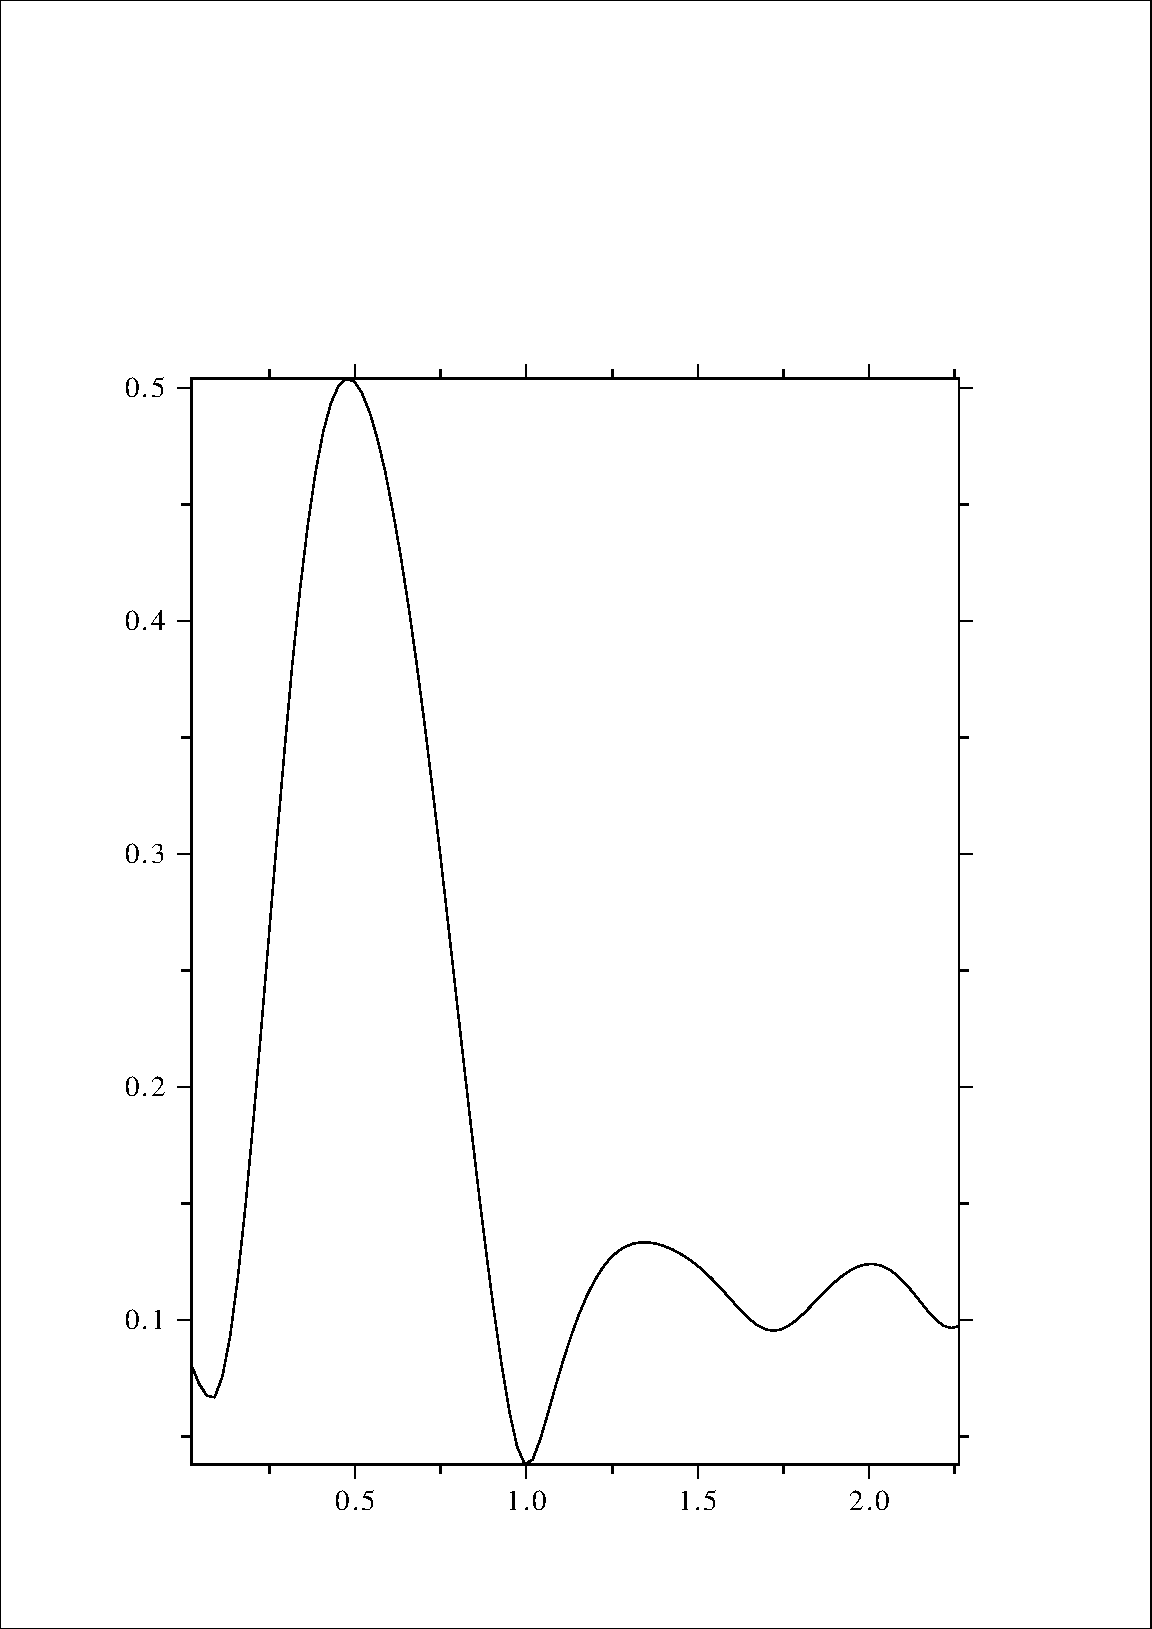
\includegraphics[scale=0.4]{RES_1s_tt1abspi.pdf}

y en $\eta=1.1$, $r=a$, 

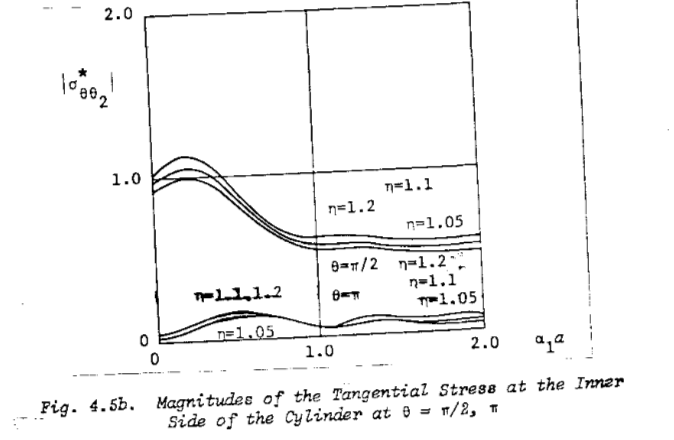
\includegraphics[scale=0.4]{res2}

en $\theta=\pi/2$ y en $\theta=\pi$ respectivamente,

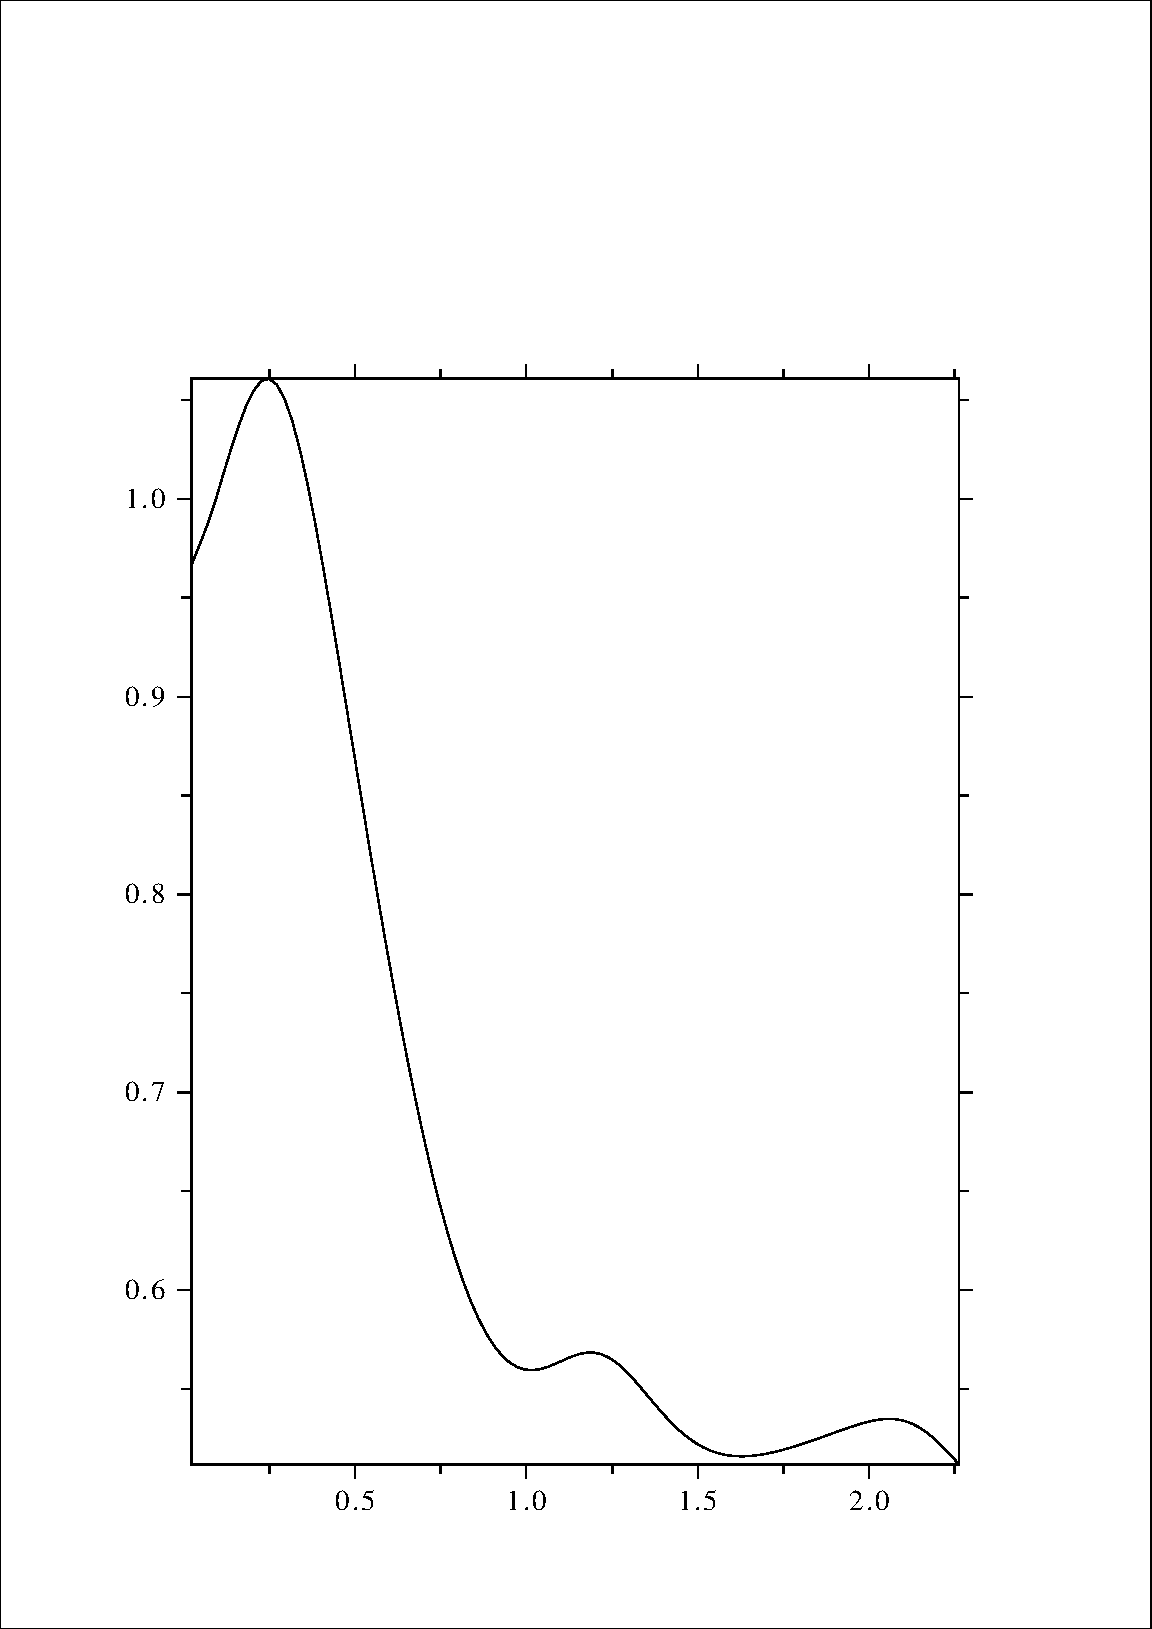
\includegraphics[scale=0.4]{RES_2s_tt2abspi2.pdf}
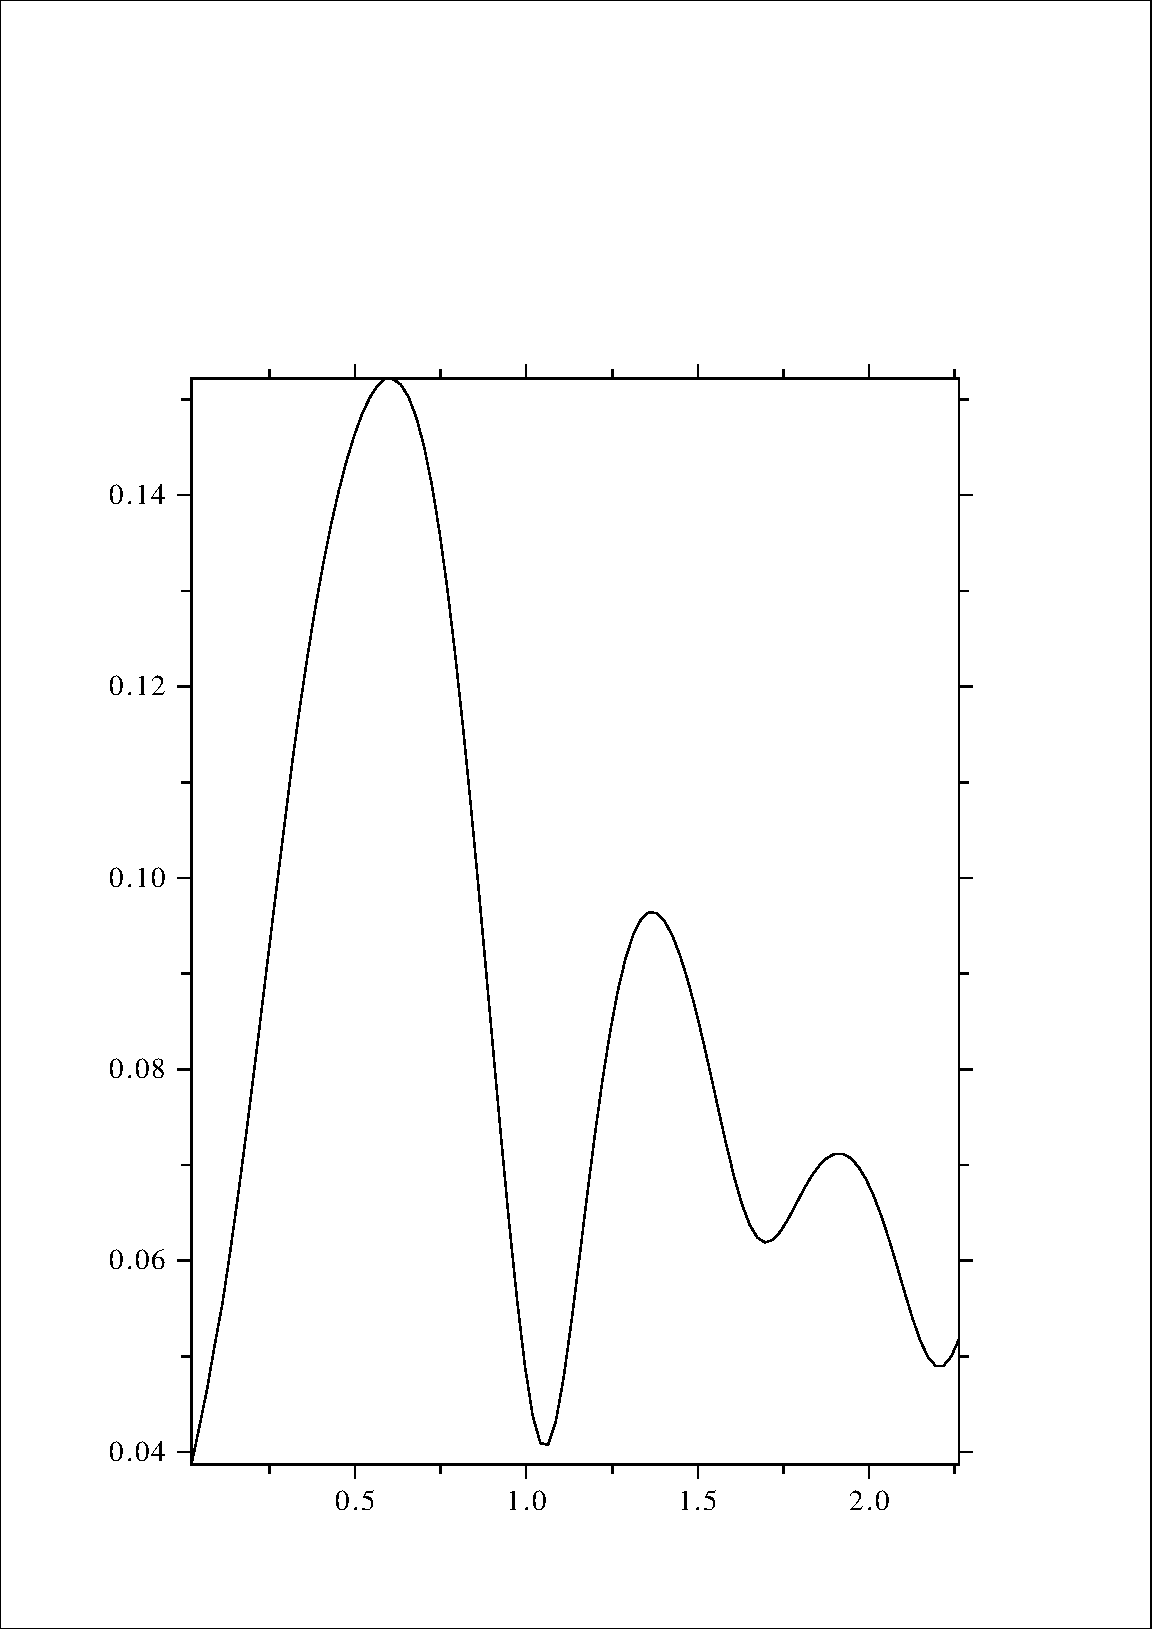
\includegraphics[scale=0.4]{RES_2s_tt2abspi.pdf}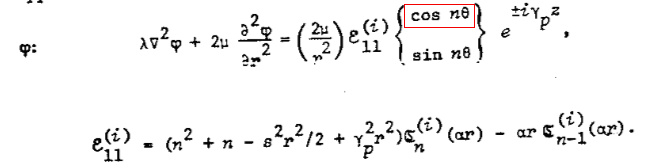
\includegraphics[scale=0.5]{e11}
\begingroup
\fontsize{10pt}{12pt}
\selectfont
\definecolor{shadecolor}{rgb}{0.925,0.925,0.925}
\begin{shaded}
\begin{verbatim}
      function e11(i,c,reg,r,n)
      use vars_func_of_w, only : alfa,s2,gammaP
      use datos, only : radios
      use Hank, only : Bess
      implicit none
      complex*16 :: e11
      integer :: i,c,reg,r,n
      complex*16, pointer :: Bess_n,Bess_n_1
!     c = 1 !alfa
      Bess_n => Bess(reg)%JYH1H2(i,n)%r(r)%c(1)
      Bess_n_1 => Bess(reg)%JYH1H2(i,n-1)%r(r)%c(1)
      e11 = (n**2 + n - s2(reg) * radios(r)**2 / 2. + & 
      gammaP**2 * radios(r)**2) * Bess_n - alfa(reg)* radios(r) * Bess_n_1
      end function e11
\end{verbatim}
\end{shaded}
\endgroup
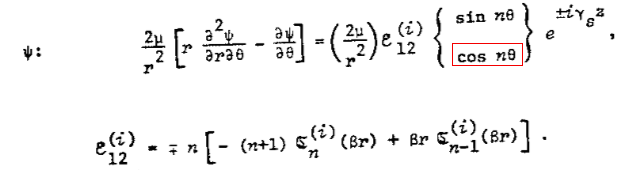
\includegraphics[scale=0.5]{e12}
\begingroup
\fontsize{10pt}{12pt}
\selectfont
\definecolor{shadecolor}{rgb}{0.925,0.925,0.925}
\begin{shaded}
\begin{verbatim}
      function e12(i,c,reg,r,n)
      use vars_func_of_w, only : beta
      use datos, only : radios
      use Hank, only : Bess
      implicit none
      complex*16 :: e12
      integer :: i,c,reg,r,n
      complex*16, pointer :: Bess_n,Bess_n_1
!     c = 2 !beta
      Bess_n => Bess(reg)%JYH1H2(i,n)%r(r)%c(2)
      Bess_n_1 => Bess(reg)%JYH1H2(i,n-1)%r(r)%c(2)
      e12 = n * (-(n+1)* Bess_n + beta(reg) * radios(r) * Bess_n_1)
      end function e12
\end{verbatim}
\end{shaded}
\endgroup
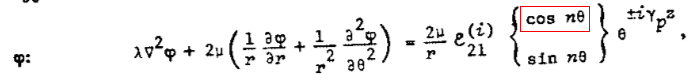
\includegraphics[scale=0.5]{e21a}

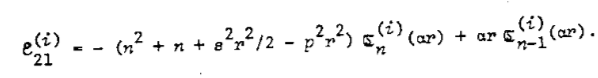
\includegraphics[scale=0.5]{e21b}
\begingroup
\fontsize{10pt}{12pt}
\selectfont
\definecolor{shadecolor}{rgb}{0.925,0.925,0.925}
\begin{shaded}
\begin{verbatim}
      function e21(i,c,reg,r,n)
      use vars_func_of_w, only : alfa,s2,p2
      use datos, only : radios
      use Hank, only : Bess
      implicit none
      complex*16 :: e21
      integer :: i,c,reg,r,n
      complex*16, pointer :: Bess_n,Bess_n_1
!     c = 1 !alfa
      Bess_n => Bess(reg)%JYH1H2(i,n)%r(r)%c(1)
      Bess_n_1 => Bess(reg)%JYH1H2(i,n-1)%r(r)%c(1)
      e21 = - (n**2 + n + s2(reg)*radios(r)**2 / 2. - p2(reg)*radios(r)**2) * &
             Bess_n + alfa(reg) * radios(r) * Bess_n_1
      end function e21
\end{verbatim}
\end{shaded}
\endgroup
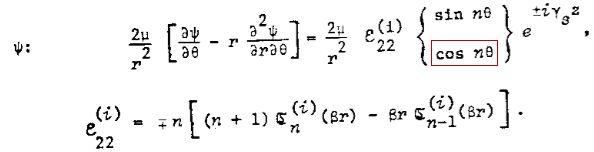
\includegraphics[scale=0.5]{e22}
\begingroup
\fontsize{10pt}{12pt}
\selectfont
\definecolor{shadecolor}{rgb}{0.925,0.925,0.925}
\begin{shaded}
\begin{verbatim}
      function e22(i,c,reg,r,n)
      use vars_func_of_w, only : beta
      use datos, only : radios
      use Hank, only : Bess
      implicit none
      complex*16 :: e22
      integer :: i,c,reg,r,n
      complex*16, pointer :: Bess_n,Bess_n_1
!     c = 2 !beta
      Bess_n => Bess(reg)%JYH1H2(i,n)%r(r)%c(2)
      Bess_n_1 => Bess(reg)%JYH1H2(i,n-1)%r(r)%c(2)
      e22 = n * ((n+1)*Bess_n - beta(reg)*radios(r)*Bess_n_1)
      end function e22
\end{verbatim}
\end{shaded}
\endgroup
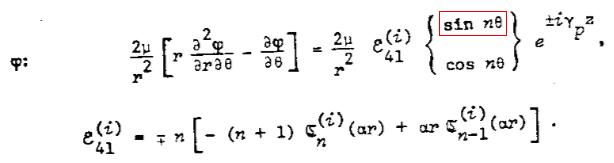
\includegraphics[scale=0.5]{e41}
\begingroup
\fontsize{10pt}{12pt}
\selectfont
\definecolor{shadecolor}{rgb}{0.925,0.925,0.925}
\begin{shaded}
\begin{verbatim}
      function e41(i,c,reg,r,n)
      use vars_func_of_w, only : alfa
      use datos, only : radios
      use Hank, only : Bess
      implicit none
      complex*16 :: e41
      integer :: i,c,reg,r,n
      complex*16, pointer :: Bess_n,Bess_n_1
!     c = 1 !alfa
      Bess_n => Bess(reg)%JYH1H2(i,n)%r(r)%c(1)
      Bess_n_1 => Bess(reg)%JYH1H2(i,n-1)%r(r)%c(1)
      e41 = - n * (-(n+1) * Bess_n + alfa(reg)*radios(r)*Bess_n_1)
      end function e41
\end{verbatim}
\end{shaded}
\endgroup
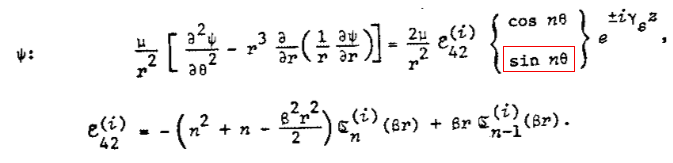
\includegraphics[scale=0.5]{e42}
\begingroup
\fontsize{10pt}{12pt}
\selectfont
\definecolor{shadecolor}{rgb}{0.925,0.925,0.925}
\begin{shaded}
\begin{verbatim}
      function e42(i,c,reg,r,n)
      use vars_func_of_w, only : beta
      use datos, only : radios
      use Hank, only : Bess
      implicit none
      complex*16 :: e42
      integer :: i,c,reg,r,n
      complex*16, pointer :: Bess_n,Bess_n_1
!     c = 2 !beta
      Bess_n => Bess(reg)%JYH1H2(i,n)%r(r)%c(2)
      Bess_n_1 => Bess(reg)%JYH1H2(i,n-1)%r(r)%c(2)
      e42 = - (n**2 + n - beta(reg)**2 * radios(r)**2 / 2.) * Bess_n + &
            beta(reg) * radios(r) * Bess_n_1
      end function e42
\end{verbatim}
\end{shaded}
\endgroup
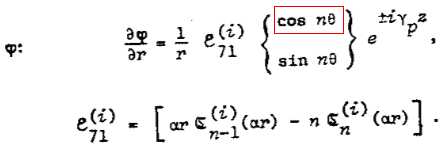
\includegraphics[scale=0.5]{e71}
\begingroup
\fontsize{10pt}{12pt}
\selectfont
\definecolor{shadecolor}{rgb}{0.925,0.925,0.925}
\begin{shaded}
\begin{verbatim}
      function e71(i,c,reg,r,n)
      use vars_func_of_w, only : alfa
      use datos, only : radios
      use Hank, only : Bess
      implicit none
      complex*16 :: e71
      integer :: i,c,reg,r,n
      complex*16, pointer :: Bess_n,Bess_n_1
!     c = 1 !alfa
      Bess_n => Bess(reg)%JYH1H2(i,n)%r(r)%c(1)
      Bess_n_1 => Bess(reg)%JYH1H2(i,n-1)%r(r)%c(1)
      e71 = alfa(reg) * radios(r) * Bess_n_1 - n * Bess_n
      end function e71
\end{verbatim}
\end{shaded}
\endgroup
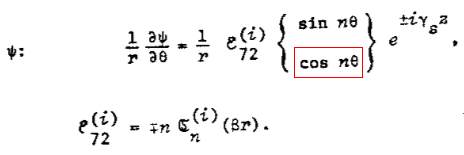
\includegraphics[scale=0.5]{e72}
\begingroup
\fontsize{10pt}{12pt}
\selectfont
\definecolor{shadecolor}{rgb}{0.925,0.925,0.925}
\begin{shaded}
\begin{verbatim}
      function e72(i,c,reg,r,n)
      use Hank, only : Bess
      implicit none
      complex*16 :: e72
      integer :: i,c,reg,r,n
      complex*16, pointer :: Bess_n
!     c = 2 !beta
      Bess_n => Bess(reg)%JYH1H2(i,n)%r(r)%c(2)
      e72 = n * Bess_n
      end function e72
\end{verbatim}
\end{shaded}
\endgroup
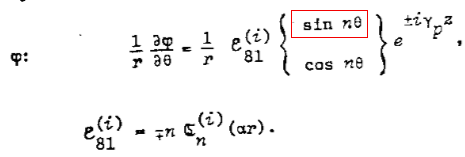
\includegraphics[scale=0.5]{e81}
\begingroup
\fontsize{10pt}{12pt}
\selectfont
\definecolor{shadecolor}{rgb}{0.925,0.925,0.925}
\begin{shaded}
\begin{verbatim}
      function e81(i,c,reg,r,n)
      use Hank, only : Bess
      implicit none
      complex*16 :: e81
      integer :: i,c,reg,r,n
      complex*16, pointer :: Bess_n
!     c = 1 !alfa
      Bess_n => Bess(reg)%JYH1H2(i,n)%r(r)%c(1)
      e81 = - n * Bess_n
      end function e81
\end{verbatim}
\end{shaded}
\endgroup
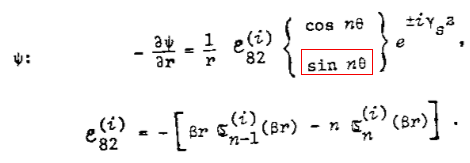
\includegraphics[scale=0.5]{e82}
\begingroup
\fontsize{10pt}{12pt}
\selectfont
\definecolor{shadecolor}{rgb}{0.925,0.925,0.925}
\begin{shaded}
\begin{verbatim}
      function e82(i,c,reg,r,n)
      use vars_func_of_w, only : beta
      use datos, only : radios
      use Hank, only : Bess
      implicit none
      complex*16 :: e82
      integer :: i,c,reg,r,n
      complex*16, pointer :: Bess_n,Bess_n_1
!     c = 2 !beta
      Bess_n => Bess(reg)%JYH1H2(i,n)%r(r)%c(2)
      Bess_n_1 => Bess(reg)%JYH1H2(i,n-1)%r(r)%c(2)
      e82 = - (beta(reg) * radios(r) * Bess_n_1 & 
              - n * Bess_n)
      end function e82
\end{verbatim}
\end{shaded}
\endgroup

\end{document}